\subsection{差分と平均変化率}

制御では、温度、位置、角度、電圧、電流のように時間とともに変わる量を扱う。連続時間の式を書く前に、まず有限な二つの時刻の差を比べる。時刻 $t_1$ の位置が $q(t_1)$、時刻 $t_2$ の位置が $q(t_2)$ なら、位置の変化量は
\begin{equation}
  \Delta q=q(t_2)-q(t_1)
\end{equation}
である。時刻の変化量は
\begin{equation}
  \Delta t=t_2-t_1
\end{equation}
である。$\Delta$ は「小さい」という意味ではなく、「後の値と前の値の差」を表す記号である。したがって、$\Delta t$ は正にも負にもなりうるが、同じ時刻どうしを比べると割り算できないので平均変化率を作るときは $\Delta t\ne0$ とする。

\begin{definition}[平均変化率]
量 $q$ が時刻 $t_1$ から $t_2$ までの時間 $\Delta t=t_2-t_1\ne0$ の間に $\Delta q=q(t_2)-q(t_1)$ だけ変化したとき、
\begin{equation}
  \frac{\Delta q}{\Delta t}
\end{equation}
を平均変化率という。
\end{definition}

平均変化率の単位は、$q$ の単位を時間の単位で割ったものである。$q$ が位置 m なら平均変化率は $\mathrm{m/s}$、角度 rad なら $\mathrm{rad/s}$、温度 $^\circ\mathrm{C}$ なら $^\circ\mathrm{C/s}$ である。次元で書けば、$q$ の次元が $Q$ なら平均変化率の次元は $QT^{-1}$ である。

たとえば $t_1=1\,\mathrm{s}$ で $q(t_1)=2\,\mathrm{m}$、$t_2=4\,\mathrm{s}$ で $q(t_2)=11\,\mathrm{m}$ なら、
\begin{align}
  \Delta q&=11-2=9\,\mathrm{m},\\
  \Delta t&=4-1=3\,\mathrm{s},\\
  \frac{\Delta q}{\Delta t}&=\frac{9\,\mathrm{m}}{3\,\mathrm{s}}=3\,\mathrm{m/s}.
\end{align}
これは、この区間における平均速度が $3\,\mathrm{m/s}$ であることを表す。

平均変化率はグラフの傾きとしても読める。横軸を $t$、縦軸を $q(t)$ とする。二つの点
\begin{equation}
  P_1=(t_1,q(t_1)),\qquad P_2=(t_2,q(t_2))
\end{equation}
を結ぶ直線を割線という。割線の傾きは
\begin{equation}
  \frac{q(t_2)-q(t_1)}{t_2-t_1}
  =\frac{\Delta q}{\Delta t}
\end{equation}
である。つまり平均変化率は、ある時間幅全体を一本の直線で見たときの傾きである。サンプリングされたデータだけがある場合、最初に計算できる変化の情報はこの割線の傾きである。

ある一つの時刻 $t_0$ での瞬間的な変化の速さを知りたいときは、比較する時刻を $t_0$ のすぐ近くに取る。$h$ を時間のずれとして $t_2=t_0+h$、$t_1=t_0$ と置くと、平均変化率は
\begin{equation}
  \frac{q(t_0+h)-q(t_0)}{h},\qquad h\ne0
\end{equation}
である。ここで $h$ を正から 0 に近づけても負から 0 に近づけても同じ有限値へ近づくなら、その値を時刻 $t_0$ における微分係数と呼ぶ。

\begin{definition}[微分係数]
関数 $q(t)$ が時刻 $t_0$ の近くで定義されているとする。極限
\begin{equation}
  \lim_{h\to0}\frac{q(t_0+h)-q(t_0)}{h}
\end{equation}
が存在するとき、$q$ は $t_0$ で微分可能であるといい、この極限値を $t_0$ における微分係数という。
\end{definition}

微分可能であるためには、$t_0$ の左右から近づけた平均変化率が同じ値へ近づく必要がある。段差のように値が飛ぶ関数や、鋭い折れ曲がりを持つ関数では、この極限が存在しない場合がある。制御工学の連続時間モデルでは、状態や入力が十分なめらかで、必要な微分が存在する範囲を仮定して式を作る。ただし実装された制御器は離散時刻でデータを受け取るので、後で差分近似とサンプリング周期の影響を別に扱う。

微分係数を時刻 $t$ の関数として並べたものを導関数と呼び、次のように書く。
\begin{equation}
  \frac{\dd q}{\dd t}(t)
  =\lim_{h\to0}\frac{q(t+h)-q(t)}{h}.
\end{equation}
本文では、時間微分を
\begin{equation}
  \dot{q}(t)=\frac{\dd q}{\dd t}(t)
\end{equation}
とも書く。点記法は、力学や状態方程式で頻繁に使う。$q$ が位置なら $\dot{q}$ は速度、$\ddot{q}$ は加速度である。

\begin{definition}[速度と加速度]
位置 $q(t)$ の時間微分
\begin{equation}
  v(t)=\dot{q}(t)=\frac{\dd q}{\dd t}(t)
\end{equation}
を速度という。速度の時間微分
\begin{equation}
  a(t)=\dot{v}(t)=\ddot{q}(t)=\frac{\dd^2 q}{\dd t^2}(t)
\end{equation}
を加速度という。
\end{definition}

$q$ の単位が m なら、速度 $v$ の単位は $\mathrm{m/s}$、加速度 $a$ の単位は $\mathrm{m/s^2}$ である。次元で書けば、位置が $L$、速度が $LT^{-1}$、加速度が $LT^{-2}$ である。質量ばねダンパ系の式
\begin{equation}
  m\ddot{q}+c\dot{q}+kq=u
\end{equation}
で、$m\ddot{q}$ が力になるのは、$\ddot{q}$ が加速度の次元を持つからである。

\begin{example}[等加速度運動から速度を取り出す]
初期位置 $q_0$、初期速度 $v_0$、一定加速度 $a_0$ を持つ直線運動を
\begin{equation}
  q(t)=q_0+v_0t+\frac{1}{2}a_0t^2
\end{equation}
と書く。時刻 $t_0$ における平均変化率を定義どおり計算する。
\begin{align}
  \frac{q(t_0+h)-q(t_0)}{h}
  &=
    \frac{
      q_0+v_0(t_0+h)+\frac{1}{2}a_0(t_0+h)^2
      -q_0-v_0t_0-\frac{1}{2}a_0t_0^2
    }{h}\\
  &=
    \frac{
      v_0h+\frac{1}{2}a_0(2t_0h+h^2)
    }{h}\\
  &=v_0+a_0t_0+\frac{1}{2}a_0h.
\end{align}
$h\to0$ とすると最後の項が消えるので、
\begin{equation}
  \dot{q}(t_0)=v_0+a_0t_0
\end{equation}
である。したがって任意の時刻で
\begin{equation}
  v(t)=v_0+a_0t
\end{equation}
となる。さらに速度を微分すると
\begin{equation}
  \dot{v}(t)
  =\lim_{h\to0}\frac{v(t+h)-v(t)}{h}
  =\lim_{h\to0}\frac{a_0h}{h}
  =a_0
\end{equation}
であり、加速度は一定値 $a_0$ である。
\end{example}

グラフで見ると、$h$ を小さくすることは、割線の二つの点を近づけることである。極限が存在するとき、割線は一点 $P_0=(t_0,q(t_0))$ で曲線に触れる直線へ近づく。この直線を接線という。接線の傾きが微分係数である。

図\ref{fig:math-entrance-examples} 左上は、この極限操作をグラフで表したものである。最初は離れた二点を結ぶ割線として平均変化率を求める。時間幅 $h$ を小さくすると、割線の傾きは一点の近くの曲がり方だけを反映するようになり、接線の傾きへ近づく。したがって、微分は二点間の傾きを一点近傍へ移す極限として定義される。

\begin{definition}[接線]
関数 $q(t)$ が $t_0$ で微分可能であるとき、点 $(t_0,q(t_0))$ を通り、傾きが $\dot{q}(t_0)$ である直線
\begin{equation}
  \ell(t)=q(t_0)+\dot{q}(t_0)(t-t_0)
\end{equation}
を、$t_0$ における $q(t)$ の接線という。
\end{definition}

接線は、曲線を時刻 $t_0$ の近くで一次関数として近似する。$h=t-t_0$ と書けば、
\begin{equation}
  q(t_0+h)\simeq q(t_0)+\dot{q}(t_0)h
\end{equation}
である。この式を接線近似、または一次近似という。正確には、微分可能な関数について
\begin{equation}
  q(t_0+h)=q(t_0)+\dot{q}(t_0)h+r(h)
\end{equation}
と書け、残り $r(h)$ は
\begin{equation}
  \lim_{h\to0}\frac{r(h)}{h}=0
\end{equation}
を満たす。つまり、十分短い時間幅では、残りの誤差は $h$ に比べて小さい。この性質が、非線形な対象を平衡点近くで線形化する考え方の入口になる。

\begin{example}[短時間の位置予測]
ある時刻 $t_0$ で位置が $q(t_0)=2.0\,\mathrm{m}$、速度が $\dot{q}(t_0)=0.3\,\mathrm{m/s}$ と測れたとする。$0.1\,\mathrm{s}$ 後の位置を接線近似で見積もると
\begin{align}
  q(t_0+0.1)
  &\simeq q(t_0)+\dot{q}(t_0)\cdot0.1\\
  &=2.0+0.3\cdot0.1\\
  &=2.03\,\mathrm{m}.
\end{align}
この計算は、短い時間だけ現在の速度が保たれるとみなす予測である。加速度が大きい場合や時間幅が長い場合には、接線近似だけでは誤差が大きくなる。
\end{example}

回転運動でも同じ定義を使う。角度を $\theta(t)$ と書くと、角度の時間微分が角速度である。

\begin{definition}[角速度と角加速度]
角度 $\theta(t)$ の時間微分
\begin{equation}
  \omega(t)=\dot{\theta}(t)=\frac{\dd \theta}{\dd t}(t)
\end{equation}
を角速度という。角速度の時間微分
\begin{equation}
  \alpha(t)=\dot{\omega}(t)=\ddot{\theta}(t)
\end{equation}
を角加速度という。
\end{definition}

角度の単位を rad、時刻の単位を s とすれば、角速度の単位は $\mathrm{rad/s}$、角加速度の単位は $\mathrm{rad/s^2}$ である。rad は弧長と半径の比なので次元としては無次元だが、回転量であることを明示するために単位記号として残す。一定角速度 $\omega_0$ で回転するなら
\begin{equation}
  \theta(t)=\theta(0)+\omega_0t
\end{equation}
であり、
\begin{equation}
  \frac{\theta(t_0+h)-\theta(t_0)}{h}
  =\frac{\omega_0h}{h}
  =\omega_0
\end{equation}
だから、瞬間角速度も $\omega_0$ である。半径 $r$ の円周上を動く点の弧長を $s(t)=r\theta(t)$ とすれば、
\begin{equation}
  \dot{s}(t)=r\dot{\theta}(t)=r\omega(t)
\end{equation}
となる。したがって、接線方向の速度の大きさは $r\omega$ である。

微分は、制御でいう状態と変化率を結ぶ。たとえば直線運動を位置と速度で表すなら、状態を二つの量の組
\begin{equation}
  x(t)=(q(t),v(t))
\end{equation}
として選べる。この並べ方は次の小節でベクトルとして定義する。このとき、状態の各成分の時間変化は
\begin{equation}
  \dot{x}(t)=(\dot{q}(t),\dot{v}(t))=(v(t),a(t))
\end{equation}
である。もし入力力 $u(t)$ が加速度を決めるなら、ニュートンの運動方程式から $m a(t)=u(t)$ として
\begin{equation}
  \dot{x}(t)=(v(t),u(t)/m)
\end{equation}
と書ける。制御器は、測った状態 $x(t)$ や出力 $y(t)$ から入力 $u(t)$ を決め、その入力が状態の時間微分 $\dot{x}(t)$ を変えることで、次の状態を変える。この「状態」と「状態の変化率」を分けて書くことが、後で現れる状態方程式
\begin{equation}
  \dot{x}(t)=f(x(t),u(t),t)
\end{equation}
の基本である。

\subsection{積分、累積量、保存則}

微分が「いまどれだけ速く変わっているか」を表すなら、積分は「その変化が時間を通してどれだけ積み上がったか」を表す。一定速度 $v$ で $\Delta t$ 秒進む距離は
\begin{equation}
  \Delta q=v\Delta t
\end{equation}
である。これは横幅が $\Delta t$、高さが $v$ の長方形の面積でもある。速度が時刻によって変わるときは、時間を細かく分け、それぞれの短い区間で速度がほぼ一定だとみなして、小さな長方形の面積を足し合わせる。この足し合わせの極限が積分である。

\begin{definition}[定積分]
関数 $r(t)$ が区間 $[t_1,t_2]$ で定義されているとする。区間を
\begin{equation}
  t_1=s_0<s_1<s_2<\cdots<s_n=t_2
\end{equation}
のように細かく分け、第 $i$ 区間の幅を $\Delta t_i=s_i-s_{i-1}$、その中で選んだ時刻を $\tau_i$ とする。和
\begin{equation}
  \sum_{i=1}^{n} r(\tau_i)\Delta t_i
\end{equation}
が、分割を十分細かくしたとき一つの値へ近づくなら、その値を
\begin{equation}
  \int_{t_1}^{t_2} r(t)\,\dd t
\end{equation}
と書き、$t_1$ から $t_2$ までの $r(t)$ の定積分という。
\end{definition}

ここで $\int$ は細かい和の極限を表す記号であり、$\dd t$ は時間方向に足し合わせることを示す。$r(t)$ が常に 0 以上なら、定積分はグラフと時間軸で囲まれた面積である。$r(t)$ が負になる区間を含むなら、時間軸より下の面積は負として数える。この意味で、定積分は符号付き面積である。

単位を見ると、積分が累積量を表すことが分かる。$r(t)$ の単位が $Q/\mathrm{s}$、時刻 $t$ の単位が s なら、
\begin{equation}
  \left[\int_{t_1}^{t_2} r(t)\,\dd t\right]
  =\frac{Q}{\mathrm{s}}\cdot\mathrm{s}
  =Q
\end{equation}
である。速度 $\mathrm{m/s}$ を時間で積分すれば位置変化 m になり、流量 $\mathrm{m^3/s}$ を時間で積分すれば体積変化 $\mathrm{m^3}$ になり、電流 $\mathrm{A}=\mathrm{C/s}$ を時間で積分すれば電荷 C になる。

\begin{example}[区分一定の速度から距離を求める]
ある移動体が、最初の $2\,\mathrm{s}$ は $1.0\,\mathrm{m/s}$、次の $3\,\mathrm{s}$ は $0.5\,\mathrm{m/s}$、最後の $1\,\mathrm{s}$ は $-0.2\,\mathrm{m/s}$ で動いたとする。速度は区間ごとに一定なので、位置変化は長方形の面積の和として
\begin{align}
  \Delta q
  &=1.0\cdot2+0.5\cdot3+(-0.2)\cdot1\\
  &=2.0+1.5-0.2\\
  &=3.3\,\mathrm{m}
\end{align}
である。最後の区間は速度が負なので、進んだ向きと逆向きの変化として差し引かれる。速度グラフの符号付き面積が位置変化になる、という読み方である。
\end{example}

\begin{figure}[tb]
\centering
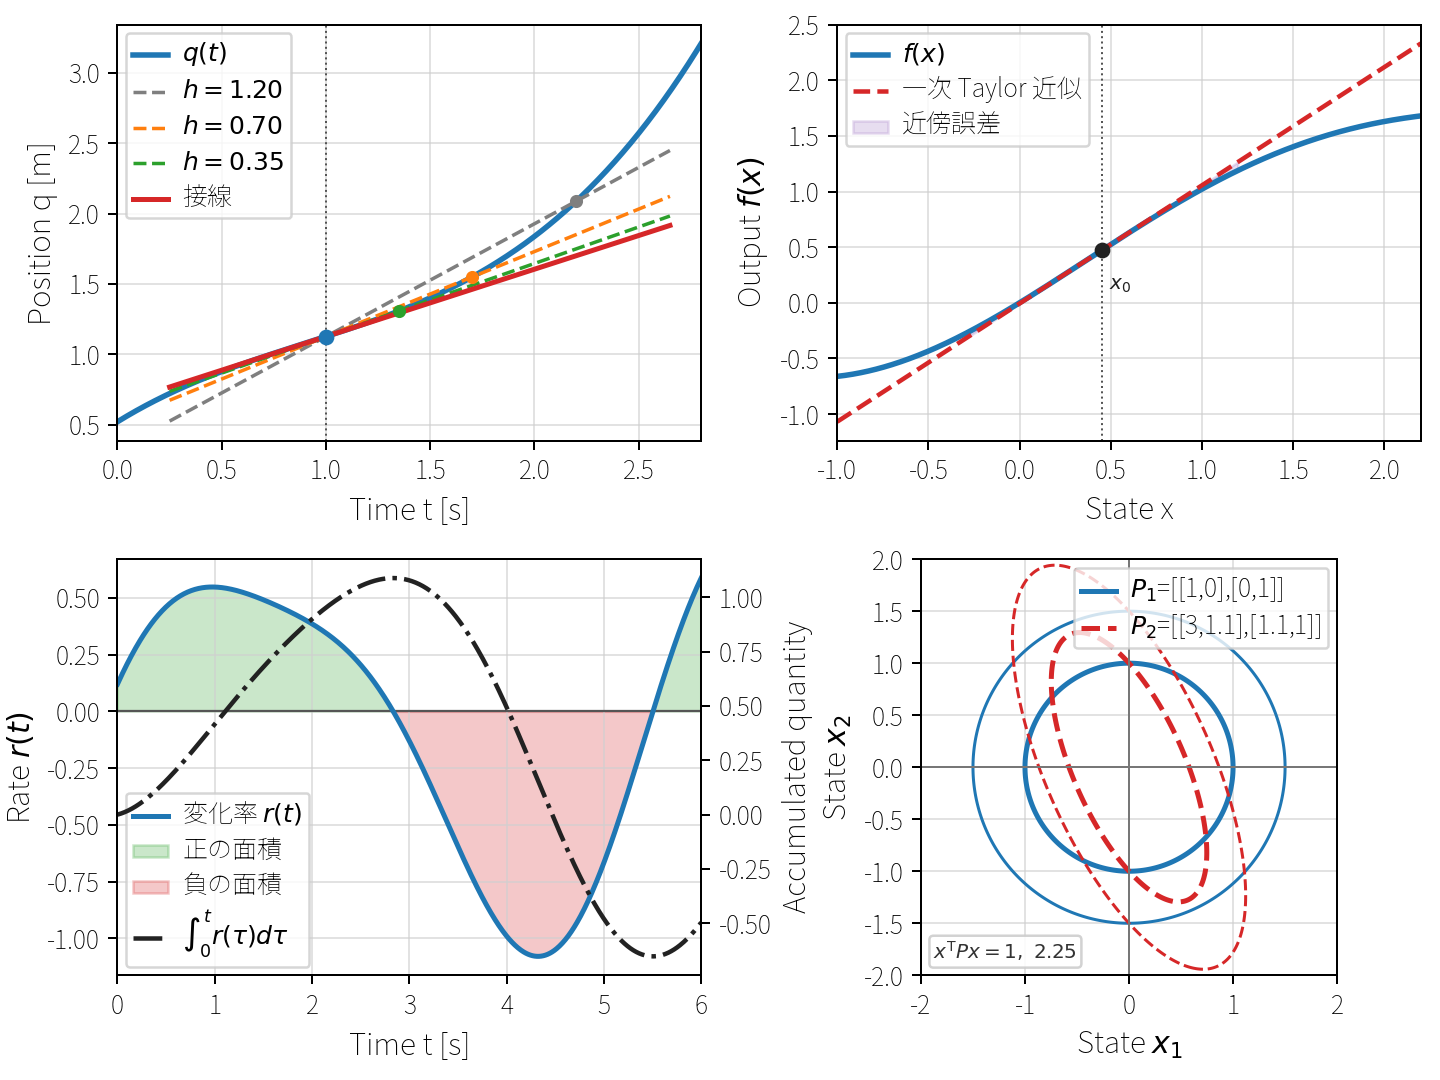
\includegraphics[width=0.94\linewidth,bb=0 0 1440 1080]{figures/math_entrance_examples.png}
\caption{微分、積分、Taylor 近似、二次形式を制御で使う前に確認する視覚例。左上は割線が接線へ近づく過程であり、平均変化率から微分係数へ進む極限を示す。左下は正負の変化率 $r(t)$ を符号付き面積として足し合わせ、その累積量が時間とともに変わる様子を示す。右上は操作点 $x_0$ での一次 Taylor 近似と真の関数との差であり、線形化の有効範囲を示す。右下は
$P_1=\begin{bmatrix}1&0\\0&1\end{bmatrix}$ と
$P_2=\begin{bmatrix}3&1.1\\1.1&1\end{bmatrix}$ が作る
$x^\T P x=1,2.25$ の等高線であり、重みが大きい方向ほど同じ値の楕円が狭くなる。}
\label{fig:math-entrance-examples}
\end{figure}

図\ref{fig:math-entrance-examples} 左下では、曲線が時間軸より上にある部分を正、下にある部分を負として足し合わせている。累積量の曲線は、正の面積が多い区間では増え、負の面積が多い区間では減る。積分を面積だけでなく状態更新として解釈する際は、この符号付き面積が蓄えの増減に対応する。

時間変化がなめらかなら、微分と積分は互いに逆向きの操作になる。位置 $q(t)$ の微分が速度 $\dot{q}(t)$ であるなら、短い時間幅 $\Delta t_i$ では
\begin{equation}
  q(s_i)-q(s_{i-1})
  \simeq \dot{q}(\tau_i)\Delta t_i
\end{equation}
と近似できる。これを $t_1$ から $t_2$ まで足すと、左辺は途中の項が打ち消し合う。
\begin{align}
  \sum_{i=1}^{n}\{q(s_i)-q(s_{i-1})\}
  &=
    \{q(s_1)-q(s_0)\}
    +\{q(s_2)-q(s_1)\}
    +\cdots
    +\{q(s_n)-q(s_{n-1})\}\\
  &=q(s_n)-q(s_0)\\
  &=q(t_2)-q(t_1).
\end{align}
分割を細かくした極限では、右辺の和が定積分になる。

\begin{formula}[微積分の基本定理]
関数 $q(t)$ が区間 $[t_1,t_2]$ で連続的に微分可能、すなわち $\dot{q}(t)$ が連続であるとき、
\begin{equation}
  q(t_2)-q(t_1)=\int_{t_1}^{t_2}\dot{q}(t)\,\dd t
\end{equation}
が成り立つ。したがって
\begin{equation}
  q(t_2)=q(t_1)+\int_{t_1}^{t_2}\dot{q}(t)\,\dd t
\end{equation}
である。
\end{formula}

この式は、制御で最もよく使う状態更新の形である。状態を $x(t)$ と書き、その時間微分が $\dot{x}(t)$ で与えられているなら、
\begin{equation}
  x(t_2)=x(t_1)+\int_{t_1}^{t_2}\dot{x}(t)\,\dd t
\end{equation}
となる。$x(t)$ が複数の成分を持つときは、各成分に同じ式を適用する。後で状態方程式を
\begin{equation}
  \dot{x}(t)=f(x(t),u(t),t)
\end{equation}
と書いたとき、入力 $u(t)$ が直接「次の状態」を与えるのではなく、まず変化率 $\dot{x}(t)$ を決め、その変化率を時間で積分して状態が更新される。

積分の形は、保存則からモデルを作るときにも現れる。保存則とは、ある量の蓄えが、入ってくる量、出ていく量、内部で作られる量、内部で消える量の差で変わるという考え方である。蓄えられた量を $S(t)$ とし、正味の流入率を $r(t)$ と書けば、
\begin{equation}
  \dot{S}(t)=r(t)
\end{equation}
であり、積分すると
\begin{equation}
  S(t_2)=S(t_1)+\int_{t_1}^{t_2}r(t)\,\dd t
\end{equation}
である。これは「変化率の式」を「蓄えの更新式」へ変える操作である。

\begin{example}[タンクの体積保存]
タンク内の水量を体積 $V(t)$ で表す。流入量を $q_{\mathrm{in}}(t)$、流出量を $q_{\mathrm{out}}(t)$ とし、どちらの単位も $\mathrm{m^3/s}$ とする。漏れや蒸発を無視すれば、体積の保存則は
\begin{equation}
  \dot{V}(t)=q_{\mathrm{in}}(t)-q_{\mathrm{out}}(t)
\end{equation}
である。したがって
\begin{equation}
  V(t_2)=V(t_1)+
  \int_{t_1}^{t_2}
  \{q_{\mathrm{in}}(t)-q_{\mathrm{out}}(t)\}\,\dd t
\end{equation}
となる。初期体積が $V(0)=0.20\,\mathrm{m^3}$、流入量が $0.0030\,\mathrm{m^3/s}$、流出量が $0.0018\,\mathrm{m^3/s}$ で $50\,\mathrm{s}$ 続くなら、
\begin{align}
  V(50)
  &=0.20+\int_{0}^{50}(0.0030-0.0018)\,\dd t\\
  &=0.20+0.0012\cdot50\\
  &=0.26\,\mathrm{m^3}.
\end{align}
断面積が一定で $A=0.50\,\mathrm{m^2}$ なら、水位 $h(t)$ は $V(t)=Ah(t)$ を満たすので、水位変化は
\begin{equation}
  \Delta h=\frac{\Delta V}{A}
  =\frac{0.06}{0.50}
  =0.12\,\mathrm{m}
\end{equation}
である。
\end{example}

熱系でも同じ構造が現れる。物体に蓄えられた熱エネルギーを $E(t)$、入る熱流を $P_{\mathrm{in}}(t)$、外へ逃げる熱流を $P_{\mathrm{out}}(t)$ とする。熱流の単位は W、すなわち $\mathrm{J/s}$ である。内部発熱などをまとめて入力側に含めれば、
\begin{equation}
  \dot{E}(t)=P_{\mathrm{in}}(t)-P_{\mathrm{out}}(t)
\end{equation}
であり、
\begin{equation}
  E(t_2)=E(t_1)+
  \int_{t_1}^{t_2}
  \{P_{\mathrm{in}}(t)-P_{\mathrm{out}}(t)\}\,\dd t
\end{equation}
となる。温度を $\theta(t)$、熱容量を $C_{\mathrm{th}}$ として $E=C_{\mathrm{th}}\theta$ と近似できる範囲では、
\begin{equation}
  C_{\mathrm{th}}\dot{\theta}(t)
  =P_{\mathrm{in}}(t)-P_{\mathrm{out}}(t)
\end{equation}
が温度の状態方程式の入口になる。

電気回路では、蓄えられる量を電荷 $Q(t)$ として同じ式を読む。電流は単位時間あたりに流れる電荷であり、単位は $\mathrm{A}=\mathrm{C/s}$ である。コンデンサへ流れ込む電流を $i(t)$ とすれば、
\begin{equation}
  \dot{Q}(t)=i(t),
  \qquad
  Q(t_2)=Q(t_1)+\int_{t_1}^{t_2}i(t)\,\dd t
\end{equation}
である。静電容量 $C$ のコンデンサでは $Q=Cv$ だから、
\begin{equation}
  C\dot{v}(t)=i(t)
\end{equation}
となる。RC 回路、熱系、タンクはいずれも、蓄えられた量の微分が正味の流入率で決まり、その微分を積分して状態が更新される、という同じ形を持つ。

\subsection{偏微分、勾配、ヤコビアン、ヘッセ行列}

状態方程式や評価関数は、一つの量だけでなく、位置、速度、温度、入力、外乱、パラメータのような複数の量に依存する。たとえば熱系の温度変化率は、現在の温度だけでなく、加える熱量や周囲温度にも依存する。制御対象を平衡点の近くで線形化するには、「一つの量を少し変え、ほかの量を固定したときに出力がどれだけ変わるか」を測る記号が必要である。そのために使うのが偏微分である。

\begin{definition}[偏微分]
関数 $f(x_1,x_2,\ldots,x_n)$ が複数の実数を入力に持つとする。点
\begin{equation}
  a=(a_1,a_2,\ldots,a_n)
\end{equation}
の近くで、$x_i$ だけを変え、ほかの変数を固定した平均変化率
\begin{equation}
  \frac{
    f(a_1,\ldots,a_i+h,\ldots,a_n)
    -f(a_1,\ldots,a_i,\ldots,a_n)
  }{h}
\end{equation}
が $h\to0$ で有限値へ近づくとき、その値を $x_i$ に関する偏微分係数といい、
\begin{equation}
  \frac{\partial f}{\partial x_i}(a)
  =
  \lim_{h\to0}
  \frac{
    f(a_1,\ldots,a_i+h,\ldots,a_n)-f(a)
  }{h}
\end{equation}
と書く。
\end{definition}

記号 $\partial$ は、複数の変数のうち一部だけを動かしていることを表す。通常の微分 $\dd/\dd t$ は入力が一つの関数に対する変化率であり、偏微分 $\partial/\partial x_i$ は多変数関数で一つの方向だけを見た変化率である。単位も通常の微分と同じ考えで決まる。$f$ の単位を $Y$、$x_i$ の単位を $X_i$ とすれば、
\begin{equation}
  \left[\frac{\partial f}{\partial x_i}\right]
  =
  \frac{Y}{X_i}
\end{equation}
である。温度 $\theta$ を W の入力 $P$ で微分した感度なら単位は $\mathrm{K/W}$、温度変化率 $\dot{\theta}$ を温度 $\theta$ で微分した係数なら単位は $1/\mathrm{s}$ になる。

\begin{example}[熱モデルの感度]
熱容量 $C_{\mathrm{th}}$、熱抵抗 $R_{\mathrm{th}}$ を持つ物体を考える。温度を $\theta(t)$、周囲温度を $\theta_{\mathrm{a}}$、加える熱入力を $P(t)$ とし、熱の逃げを $(\theta-\theta_{\mathrm{a}})/R_{\mathrm{th}}$ で近似すると、
\begin{equation}
  C_{\mathrm{th}}\dot{\theta}
  =
  P-\frac{\theta-\theta_{\mathrm{a}}}{R_{\mathrm{th}}}
\end{equation}
である。したがって温度変化率を
\begin{equation}
  f(\theta,P)
  =
  \dot{\theta}
  =
  \frac{1}{C_{\mathrm{th}}}
  \left(P-\frac{\theta-\theta_{\mathrm{a}}}{R_{\mathrm{th}}}\right)
\end{equation}
と書ける。$P$ の単位は W、$C_{\mathrm{th}}$ の単位は $\mathrm{J/K}$、$R_{\mathrm{th}}$ の単位は $\mathrm{K/W}$ である。このとき
\begin{align}
  \frac{\partial f}{\partial \theta}
  &=
  -\frac{1}{C_{\mathrm{th}}R_{\mathrm{th}}},\\
  \frac{\partial f}{\partial P}
  &=
  \frac{1}{C_{\mathrm{th}}}
\end{align}
である。$C_{\mathrm{th}}R_{\mathrm{th}}$ の単位は
\begin{equation}
  \frac{\mathrm{J}}{\mathrm{K}}\cdot
  \frac{\mathrm{K}}{\mathrm{W}}
  =
  \frac{\mathrm{J}}{\mathrm{J/s}}
  =
  \mathrm{s}
\end{equation}
だから、$\partial f/\partial\theta$ の単位は $1/\mathrm{s}$ である。また、$\partial f/\partial P=1/C_{\mathrm{th}}$ の単位は $\mathrm{K/J}$ であり、入力変化 $\Delta P$ の単位 $\mathrm{J/s}$ を掛けると $\mathrm{K/s}$ になる。これは $\dot{\theta}$ の単位と一致する。
\end{example}

複数の変数を同時に少し変えるとき、偏微分を成分として並べると一次近似を短く書ける。次の小節で正式にベクトルを定義するが、ここでは変化量を
\begin{equation}
  \Delta x=
  \begin{bmatrix}
    \Delta x_1\\
    \Delta x_2\\
    \vdots\\
    \Delta x_n
  \end{bmatrix}
\end{equation}
のように縦に並べたものとして読む。

\begin{definition}[勾配]
実数値関数 $f(x_1,\ldots,x_n)$ の偏微分を縦に並べたもの
\begin{equation}
  \nabla f(a)
  =
  \begin{bmatrix}
    \frac{\partial f}{\partial x_1}(a)\\
    \frac{\partial f}{\partial x_2}(a)\\
    \vdots\\
    \frac{\partial f}{\partial x_n}(a)
  \end{bmatrix}
\end{equation}
を、点 $a$ における $f$ の勾配という。
\end{definition}

勾配は、各入力方向に対する感度をまとめた量である。小さな変化 $\Delta x_i$ に対して、各方向の寄与を足すと
\begin{equation}
  f(a+\Delta x)-f(a)
  \simeq
  \sum_{i=1}^{n}
  \frac{\partial f}{\partial x_i}(a)\Delta x_i
\end{equation}
となる。この和は勾配を使って
\begin{equation}
  f(a+\Delta x)
  \simeq
  f(a)+(\nabla f(a))^\T \Delta x
\end{equation}
と書ける。右辺の各項はすべて $f$ と同じ単位を持つ。実際、$\partial f/\partial x_i$ の単位は $[f]/[x_i]$ であり、これに $\Delta x_i$ の単位 $[x_i]$ を掛けると $[f]$ になる。

\begin{formula}[多変数の一次テイラー展開]
関数 $f$ が点 $a$ の近くで連続的な偏微分を持ち、$\Delta x$ が十分小さいとする。このとき
\begin{equation}
  f(a+\Delta x)
  =
  f(a)+(\nabla f(a))^\T \Delta x+r_1(\Delta x)
\end{equation}
と書ける。残り $r_1(\Delta x)$ は、$\Delta x$ の大きさに比べて小さい高次の誤差である。一次近似ではこの残りを無視する。
\end{formula}

図\ref{fig:math-entrance-examples} 右上では、操作点 $x_0$ における一次 Taylor 近似を破線で示している。$x$ が $x_0$ に近い範囲では真の曲線との差が小さいが、離れるにつれて差が大きくなる。平衡点まわりの線形化も同じで、ヤコビアンから得た一次式は近傍の感度を表すが、操作点から大きく外れた応答を保証するものではない。

熱モデルを平衡点 $(\theta_0,P_0)$ の近くで見ると、偏差
\begin{equation}
  \Delta\theta=\theta-\theta_0,
  \qquad
  \Delta P=P-P_0
\end{equation}
に対して
\begin{equation}
  \Delta\dot{\theta}
  \simeq
  -\frac{1}{C_{\mathrm{th}}R_{\mathrm{th}}}\Delta\theta
  +\frac{1}{C_{\mathrm{th}}}\Delta P
\end{equation}
となる。これは非線形ではない例だが、線形化の読み方を最も単純に示している。温度が平衡点より高ければ第一項が負になり温度変化率を下げ、入力熱を増やせば第二項が正になり温度変化率を上げる。係数の単位はそれぞれ $\mathrm{K/s}$ へそろう。

出力が一つではなく複数ある場合もある。状態方程式では、状態の各成分の時間微分を同時に扱うので、出力も複数である。このとき偏微分を長方形に並べたものがヤコビアンである。

\begin{definition}[ヤコビアン]
関数
\begin{equation}
  g(x)=
  \begin{bmatrix}
    g_1(x)\\
    g_2(x)\\
    \vdots\\
    g_m(x)
  \end{bmatrix},
  \qquad
  x=(x_1,\ldots,x_n)
\end{equation}
を考える。$i$ 番目の出力 $g_i$ を $j$ 番目の入力 $x_j$ で偏微分した値を $(i,j)$ 成分として並べた行列
\begin{equation}
  J_g(a)
  =
  \begin{bmatrix}
    \frac{\partial g_1}{\partial x_1}(a)&
    \frac{\partial g_1}{\partial x_2}(a)&
    \cdots&
    \frac{\partial g_1}{\partial x_n}(a)\\
    \frac{\partial g_2}{\partial x_1}(a)&
    \frac{\partial g_2}{\partial x_2}(a)&
    \cdots&
    \frac{\partial g_2}{\partial x_n}(a)\\
    \vdots&\vdots&\ddots&\vdots\\
    \frac{\partial g_m}{\partial x_1}(a)&
    \frac{\partial g_m}{\partial x_2}(a)&
    \cdots&
    \frac{\partial g_m}{\partial x_n}(a)
  \end{bmatrix}
\end{equation}
を、点 $a$ における $g$ のヤコビアンという。
\end{definition}

ヤコビアンの $(i,j)$ 成分の単位は $[g_i]/[x_j]$ である。したがって、$J_g(a)\Delta x$ の $i$ 番目の成分は
\begin{equation}
  \sum_{j=1}^{n}
  \frac{\partial g_i}{\partial x_j}(a)\Delta x_j
\end{equation}
であり、すべて $g_i$ と同じ単位を持つ。ベクトル値関数の一次近似は
\begin{equation}
  g(a+\Delta x)
  \simeq
  g(a)+J_g(a)\Delta x
\end{equation}
である。

状態方程式を
\begin{equation}
  \dot{x}=f(x,u)
\end{equation}
と書くと、平衡点 $(x_0,u_0)$ の近くでは偏差 $\Delta x=x-x_0$、$\Delta u=u-u_0$ に対して
\begin{equation}
  \Delta\dot{x}
  \simeq
  A\Delta x+B\Delta u
\end{equation}
と近似する。ここで
\begin{equation}
  A=
  \left.\frac{\partial f}{\partial x}\right|_{(x_0,u_0)},
  \qquad
  B=
  \left.\frac{\partial f}{\partial u}\right|_{(x_0,u_0)}
\end{equation}
であり、$A$ と $B$ はそれぞれ状態と入力に関するヤコビアンである。これが局所線形化の基本形である。後で非線形モデルを扱うとき、$A$ の固有値が平衡点近くの自然な動きを決め、$B$ が入力でどの方向へ状態変化を動かせるかを表す。

最適化では、一次近似だけでなく、曲がり方も重要になる。評価関数が谷の形をしていれば最小値を持ちやすく、山や鞍点の形をしていれば同じ停留条件でも最小とは限らない。この曲がり方を表すのがヘッセ行列である。

\begin{definition}[ヘッセ行列]
実数値関数 $f(x_1,\ldots,x_n)$ の二階偏微分を並べた行列
\begin{equation}
  \nabla^2 f(a)
  =
  \begin{bmatrix}
    \frac{\partial^2 f}{\partial x_1^2}(a)&
    \frac{\partial^2 f}{\partial x_1\partial x_2}(a)&
    \cdots&
    \frac{\partial^2 f}{\partial x_1\partial x_n}(a)\\
    \frac{\partial^2 f}{\partial x_2\partial x_1}(a)&
    \frac{\partial^2 f}{\partial x_2^2}(a)&
    \cdots&
    \frac{\partial^2 f}{\partial x_2\partial x_n}(a)\\
    \vdots&\vdots&\ddots&\vdots\\
    \frac{\partial^2 f}{\partial x_n\partial x_1}(a)&
    \frac{\partial^2 f}{\partial x_n\partial x_2}(a)&
    \cdots&
    \frac{\partial^2 f}{\partial x_n^2}(a)
  \end{bmatrix}
\end{equation}
を、点 $a$ における $f$ のヘッセ行列という。
\end{definition}

ヘッセ行列の $(i,j)$ 成分の単位は $[f]/([x_i][x_j])$ である。二階偏微分が連続であれば、混合偏微分は
\begin{equation}
  \frac{\partial^2 f}{\partial x_i\partial x_j}
  =
  \frac{\partial^2 f}{\partial x_j\partial x_i}
\end{equation}
となる。この性質により、ヘッセ行列は対称になる。対称な行列の曲率は、後で二次形式や正定値を学ぶときに詳しく読む。

\begin{formula}[多変数の二次テイラー展開]
関数 $f$ が点 $a$ の近くで連続的な二階偏微分を持ち、$\Delta x$ が十分小さいとする。このとき
\begin{equation}
  f(a+\Delta x)
  =
  f(a)+(\nabla f(a))^\T \Delta x
  +\frac{1}{2}\Delta x^\T \nabla^2 f(a)\Delta x
  +r_2(\Delta x)
\end{equation}
と書ける。残り $r_2(\Delta x)$ は、$\Delta x$ の二乗に比べて小さい高次の誤差である。二次近似ではこの残りを無視する。
\end{formula}

最適化では、評価関数 $J(x)$ を小さくする $x$ を探す。一次テイラー展開から、微小変化 $\Delta x$ による評価の変化は
\begin{equation}
  \Delta J
  \simeq
  (\nabla J(x))^\T \Delta x
\end{equation}
である。したがって、$\nabla J(x)\ne0$ なら、勾配と逆向きに少し動くと $J$ は減少する。候補点でどの小さな方向にも一次の増減が残らないためには
\begin{equation}
  \nabla J(x^\ast)=0
\end{equation}
が必要である。この条件を一階の最適性条件という。ただし、これだけでは最小値とは限らない。二次テイラー展開の二次項
\begin{equation}
  \frac{1}{2}\Delta x^\T \nabla^2 J(x^\ast)\Delta x
\end{equation}
がすべての $0$ でない小さな変化 $\Delta x$ に対して正なら、点 $x^\ast$ の近くで評価は上へ曲がり、局所最小と判定できる。

\begin{example}[二乗評価の曲率]
偏差 $e$ と入力 $u$ を同時に小さくしたいとき、
\begin{equation}
  J(e,u)=q e^2+r u^2,\qquad q>0,\quad r>0
\end{equation}
という二乗評価を使う。$e$ の単位が K、$u$ の単位が W で、$J$ を無次元にしたいなら、$q$ の単位は $1/\mathrm{K^2}$、$r$ の単位は $1/\mathrm{W^2}$ である。偏微分は
\begin{align}
  \frac{\partial J}{\partial e}&=2qe,\\
  \frac{\partial J}{\partial u}&=2ru
\end{align}
なので、勾配は
\begin{equation}
  \nabla J(e,u)
  =
  \begin{bmatrix}
    2qe\\
    2ru
  \end{bmatrix}
\end{equation}
である。さらに二階偏微分を並べると
\begin{equation}
  \nabla^2 J(e,u)
  =
  \begin{bmatrix}
    2q&0\\
    0&2r
  \end{bmatrix}
\end{equation}
となる。$q,r>0$ なので、$e$ 方向にも $u$ 方向にも評価は上へ曲がる。交差項 $2s e u$ を含む評価では、ヘッセ行列の非対角成分が $e$ と $u$ の同時変化に対する曲率を表す。
\end{example}

制御で頻繁に現れる二次評価
\begin{equation}
  J(x)=x^\T P x
\end{equation}
も同じ考えで読む。$P$ が対称であるとき、勾配は $2Px$、ヘッセ行列は $2P$ である。したがって、$P$ は状態偏差の大きさを罰する重みであると同時に、評価関数の曲率を決める行列でもある。LQR、カルマンフィルタ、MPC では、この「一次項は線形化を与え、二次項は曲率と重みを与える」という見方を繰り返し使う。
